\subsection{Differential branching fraction}
\label{sec:kpimm:bf}
 
The differential branching fraction of the decay \BdToKpimm in a \qsq bin of width $(q^{2}_{\text{max}} - q^{2}_{\text{min}})$ is estimated by normalising the \BdToKpimm yield, $N_{\kpimm}$, to the total event yield of the \BdToJPsiKst control sample, $N_{\jpsi\Kstarz}$, correcting for the relative efficiency between the two decays, $\varepsilon_{\jpsi\Kstarz}/\varepsilon_{\kpimm}$,
 
\begin{equation}
\begin{split}
\frac{\deriv\BF}{\deriv\qsq} = \frac{1}{(q^{2}_{\text{max}} - q^{2}_{\text{min}}) }&f_{\KstP}\BF(\BdToJPsiKstP)\BF(\decay{\jpsi}{\mumu}) \\
\times&\BF(\decay{\KstP}{\Kp\pim})\frac{N_{\kpimm}}{(1-F_{\rm S}^{\jpsi\Kstarz})N_{\jpsi\Kstarz}} \frac{\varepsilon_{\jpsi\Kstarz}}{\varepsilon_{\kpimm}}.
\end{split}
\label{eqn:dbfdq2}
\end{equation}
 
\noindent The number of \BdToJPsiKst and \BdToKpimm candidates are obtained from unbinned maximum likelihood fits to their respective $\mkpimm$ distributions, as described in Sec.~\ref{sec:kpimm:massfit}. The number of \BdToJPsiKst candidates has to be corrected for the S-wave fraction within the narrow $\mkpi$ window of \BdToJPsiKst decays, $F_{\rm S}^{\jpsi\Kstarz}$. The value of $F_{\rm S}^{\jpsi\Kstarz}$ is obtained from Ref.~\cite{LHCb-JpsiKstar} and is adjusted to the $\mkpi$ range $796<\mkpi<996~\mevcc$. The branching fractions $\BF(\BdToJPsiKstP)$, $\BF(\decay{\jpsi}{\mumu})$ and $\BF(\decay{\KstP}{\Kp\pim})$ are $(1.19\pm0.01\pm0.08)\times10^{-3}$~\cite{belle-z-paper}, $(5.961 \pm 0.033) \times 10^{-2}$~\cite{pdg} and 2/3, respectively. The fraction $f_{\KstP}$ is used to scale the value of $\BF(\BdToJPsiKstP)$ to the correct \mkpi range.  The value of $f_{\KstP}$ is calculated by integrating the $\KstP$ lineshape given in Ref.~\cite{belle-z-paper} over the range $796<\mkpi<996~\mevcc$.
 
\subsubsection{Efficiencies and yields}

To avoid making any assumption on the unknown angular distribution of the \BdToKpimm decay, the candidate efficiency provided by the acceptance function, described in Sec.~\ref{sec:kpimm:acceptance}, is used to evaluate the average efficiency for both the \BdToJPsiKst candidates and the signal candidates in each \qsq bin.
 
If there were only signal candidates present, the average efficiency would simply be calculated as

\begin{equation}
\overline{\varepsilon} = \frac{1}{N}\sum\limits_{i}^{N}\varepsilon_{i},
\label{eqn:average_eff}
\end{equation}
 
\noindent where $\varepsilon_{i}$ is the candidate efficiency and $N$ is the number of candidates.  An estimate for the error on the average efficiency would be given by
 
\begin{equation}
\delta_{\overline{\varepsilon}} = \sqrt{\frac{1}{N(N-1)}\sum\limits_{i}^{N}(\varepsilon_{i}-\overline{\varepsilon})^{2}}.
\end{equation}
 
\noindent Due to the presence of background, the average efficiency calculated in the signal mass window will be an admixture of the average efficiency for both signal candidates ($\overline{\varepsilon}_{sig}$) and background candidates ($\overline{\varepsilon}_{bkg}$),
 
\begin{equation}
\overline{\varepsilon}_{mix} = \frac{N_{sig}\overline{\varepsilon}_{sig} + N_{bkg}\overline{\varepsilon}_{bkg}}{N_{sig}+N_{bkg}},
\end{equation}
 
\noindent where $N_{sig}$ and $N_{bkg}$ are the number of signal and background candidates in the signal mass window, respectively. This can be rearranged to give the average efficiency for the signal candidates,
 
\begin{equation}
\overline{\varepsilon}_{sig} = \frac{(N_{sig}+N_{bkg})\overline{\varepsilon}_{mix} -  N_{bkg}\overline{\varepsilon}_{bkg}}{N_{sig}}.
\end{equation}
 
\noindent However, what is needed for both the \BdToKpimm and \BdToJPsiKst modes is the ratio $N_{sig}/\overline{\varepsilon}_{sig}$.  This is given by
 
\begin{equation}
\frac{N_{sig}}{\overline{\varepsilon}_{sig}} = \frac{N_{sig}^{2}}{(N_{sig}+N_{bkg})\overline{\varepsilon}_{mix} -  N_{bkg}\overline{\varepsilon}_{bkg}},
\end{equation}
 
\noindent where the errors are propagated as
 
\begin{equation}
\begin{aligned}
\sigma_{N_{sig}/\overline{\varepsilon}_{sig}}^{2} =&
\left(\frac{N_{sig}^{2}(N_{sig}+N_{bkg})}{((N_{sig}+N_{bkg})\overline{\varepsilon}_{mix} -  N_{bkg}\overline{\varepsilon}_{bkg})^2}\right)^{2}\sigma_{\overline{\varepsilon}_{mix}}^{2}\\
+& \left(\frac{N_{sig}^{2}N_{bkg}}{((N_{sig}+N_{bkg})\overline{\varepsilon}_{mix} -  N_{bkg}\overline{\varepsilon}_{bkg})^2}\right)^{2}\sigma_{\overline{\varepsilon}_{bkg}}^{2}\\
+& \left(\frac{N_{sig}^{2}\overline{\varepsilon}_{mix}}{((N_{sig}+N_{bkg})\overline{\varepsilon}_{mix} -  N_{bkg}\overline{\varepsilon}_{bkg})^2} - \frac{2N_{sig}}{((N_{sig}+N_{bkg})\overline{\varepsilon}_{mix} -  N_{bkg}\overline{\varepsilon}_{bkg})} \right)^{2}\sigma_{N_{sig}}^{2}\\
+& \left(\frac{N_{sig}^{2}(\overline{\varepsilon}_{mix} - \overline{\varepsilon}_{bkg})}{((N_{sig}+N_{bkg})\overline{\varepsilon}_{mix} -  N_{bkg}\overline{\varepsilon}_{bkg})^2}\right)^{2}\sigma_{N_{bkg}}^{2}.
\end{aligned}
\end{equation}
 
The signal region is defined as $5230<\mkpimm<5330$~\mevcc and the background region as $5350<\mkpimm<5700$~\mevcc. For the resonant mode, the background region is altered to $5450<\mkpimm<5700$~\mevcc in order to prevent any potential pollution from \BdToJPsiKst or \BsToJPsiKst candidates.

\subsubsection{Toy studies}
 
Toy studies are performed for the extraction of $N_{sig}/\overline{\varepsilon}_{sig}$ with different numbers of signal and background candidates.  In each toy $N_{sig}$ and $N_{bkg}$ are Poisson fluctuated.  The nominal mass models, described in Sec.~\ref{sec:kpimm:massfit}, are used to generate signal and background candidates. The efficiencies for both signal and background are sampled from two gaussian functions with different means.  The pull plots for the extraction of $N_{sig}/\overline{\varepsilon}_{sig}$ are shown in Fig.~\ref{fig:bf:pulls}. No bias is observed.
 
\begin{figure}[!tb]
 \centering
 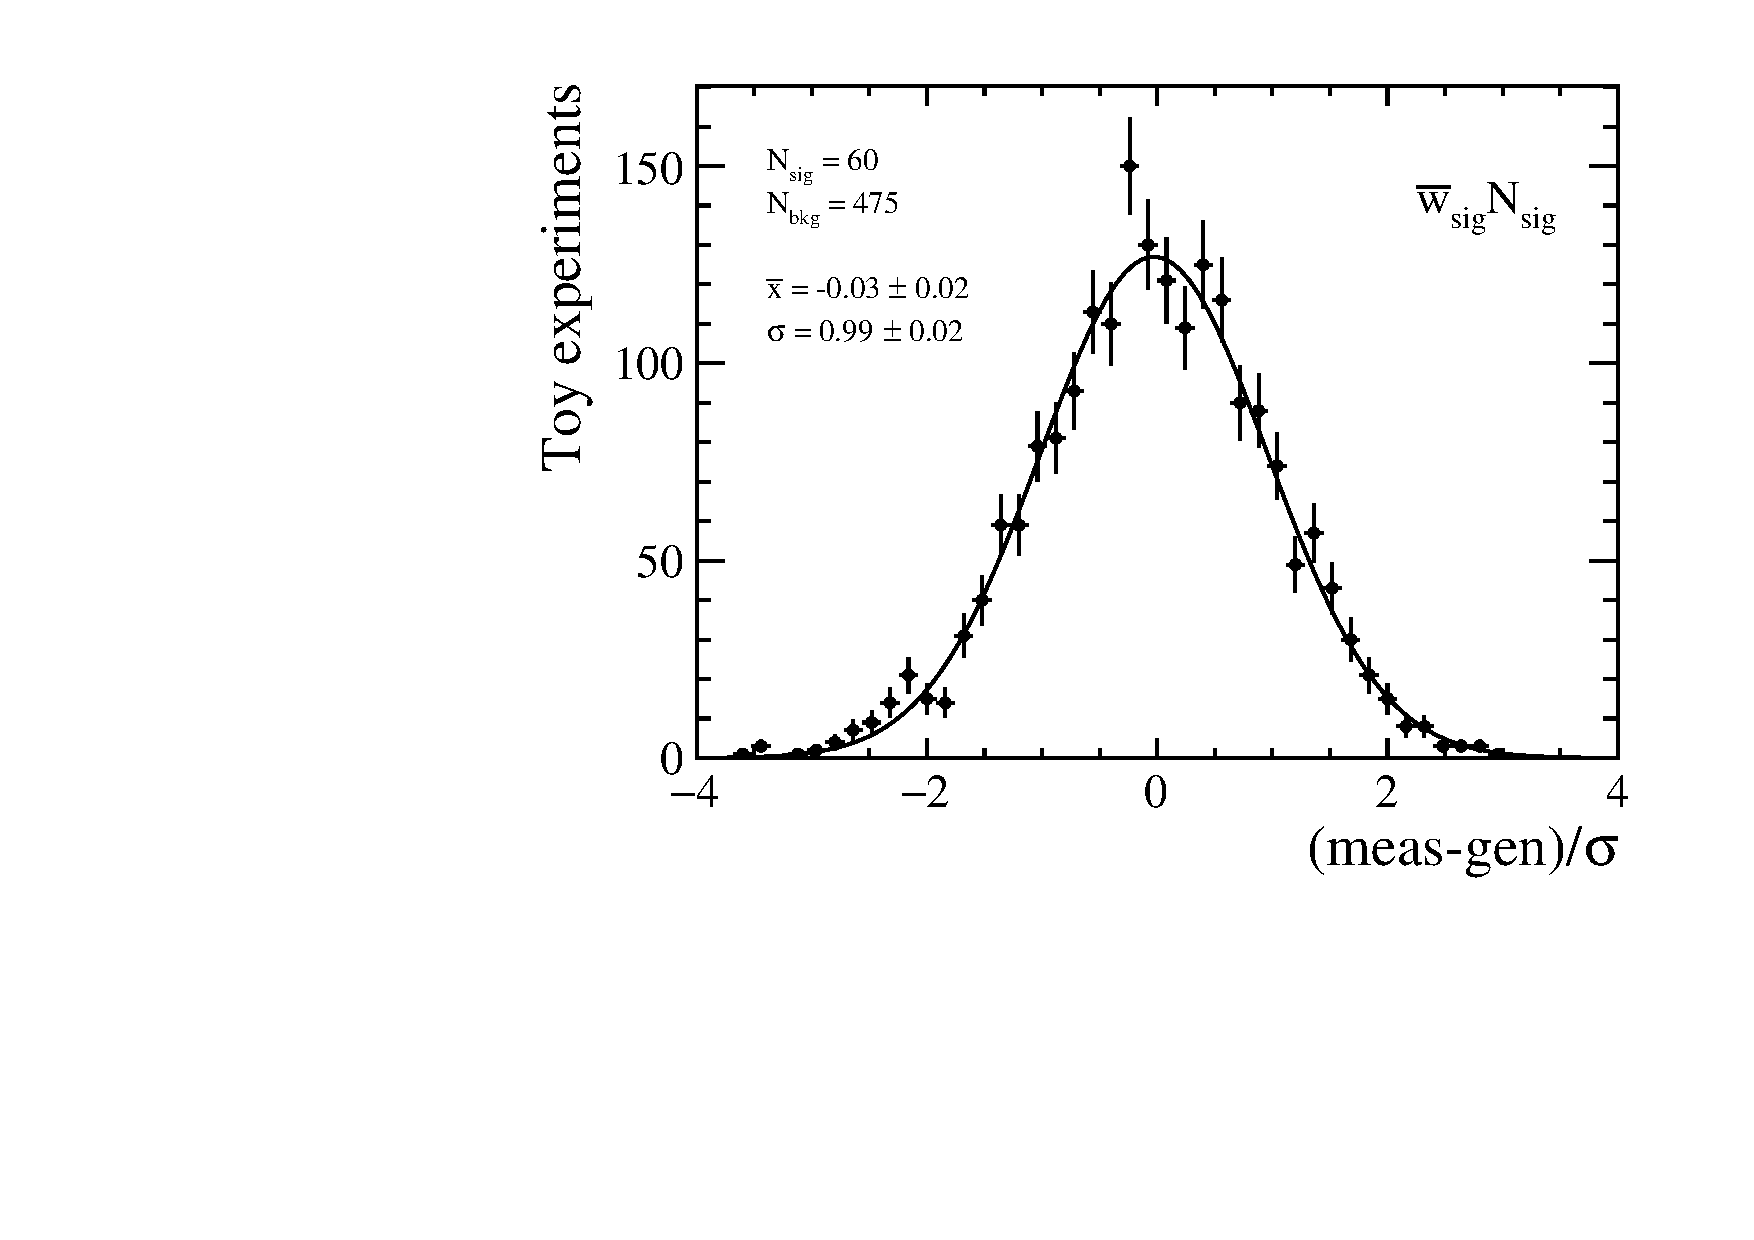
\includegraphics[width=0.45\textwidth]{figs/kpimm/bf/n_prime_low_yield.pdf}
 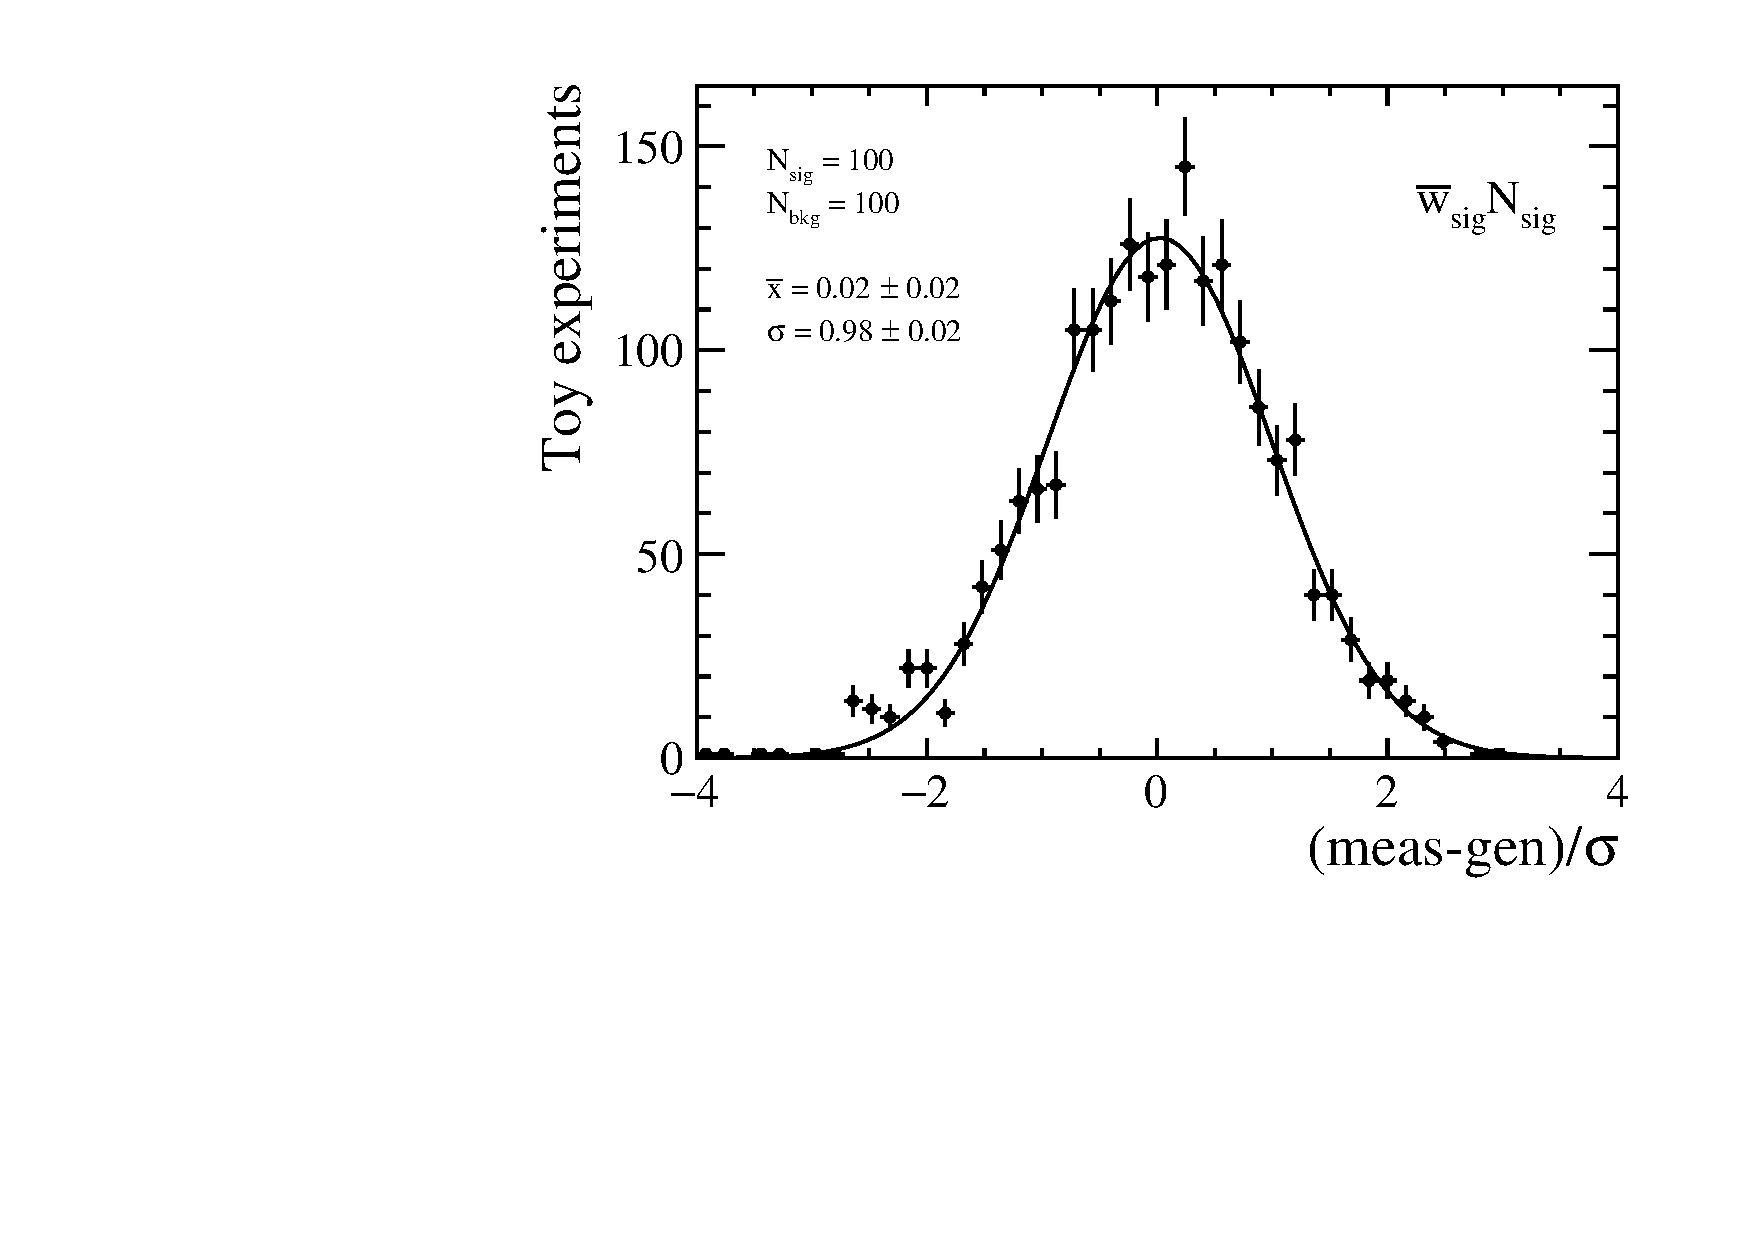
\includegraphics[width=0.45\textwidth]{figs/kpimm/bf/n_prime_med_yield.pdf}
 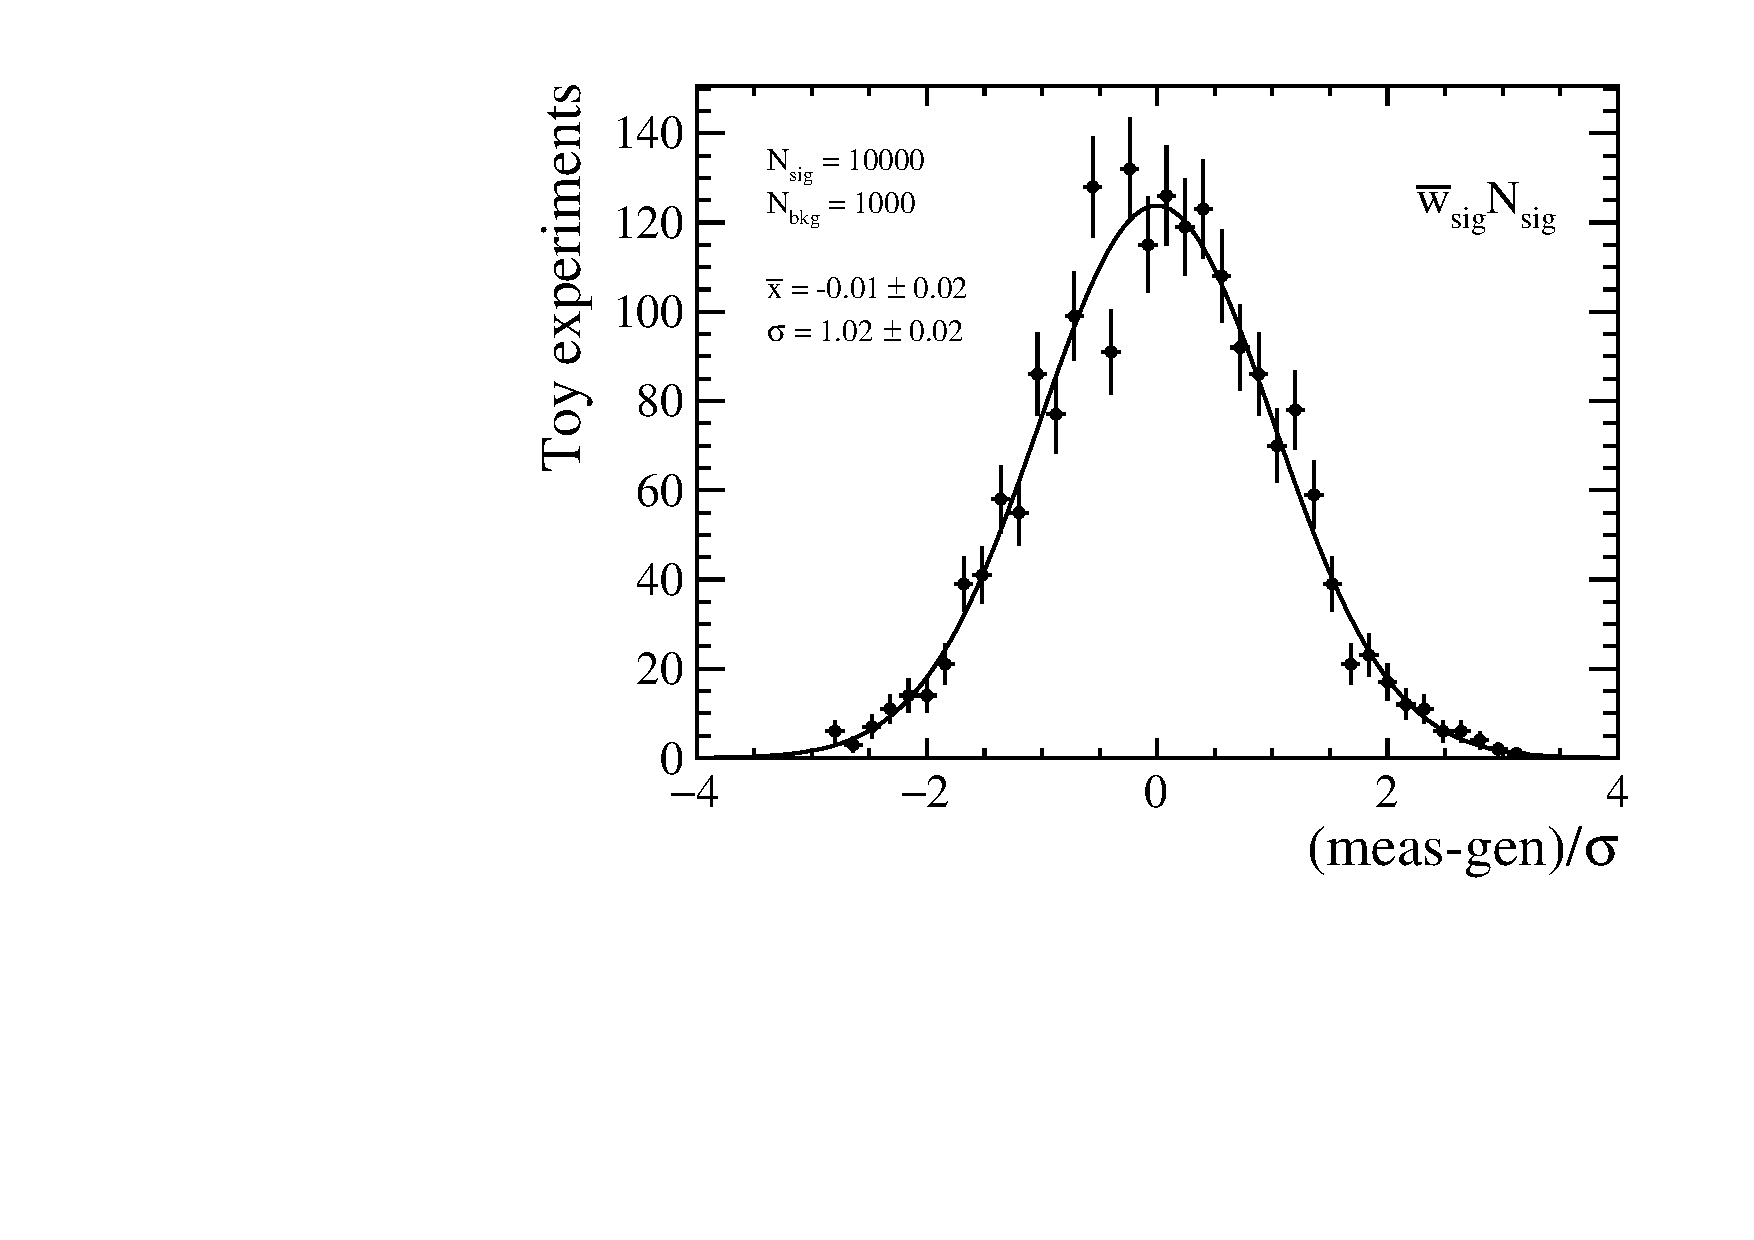
\includegraphics[width=0.45\textwidth]{figs/kpimm/bf/n_prime_high_yield.pdf}
 \caption{Pull plots for the extraction of $N_{sig}/\overline{\varepsilon}_{sig}$ with different numbers of signal and background candidates.}
 \label{fig:bf:pulls}
\end{figure}

\subsubsection{Results}

The results for the differential branching fraction are given in Fig.~\ref{fig:bf}.  The uncertainties shown are the quadratic sum of the statistical and systematic uncertainties.  The results are also presented in Table~\ref{tab:bf}.  The various sources of the systematic uncertainties are described in Sec.~\ref{sec:kpimm:systematics}.
 
\begin{figure}[!tb]
\centering
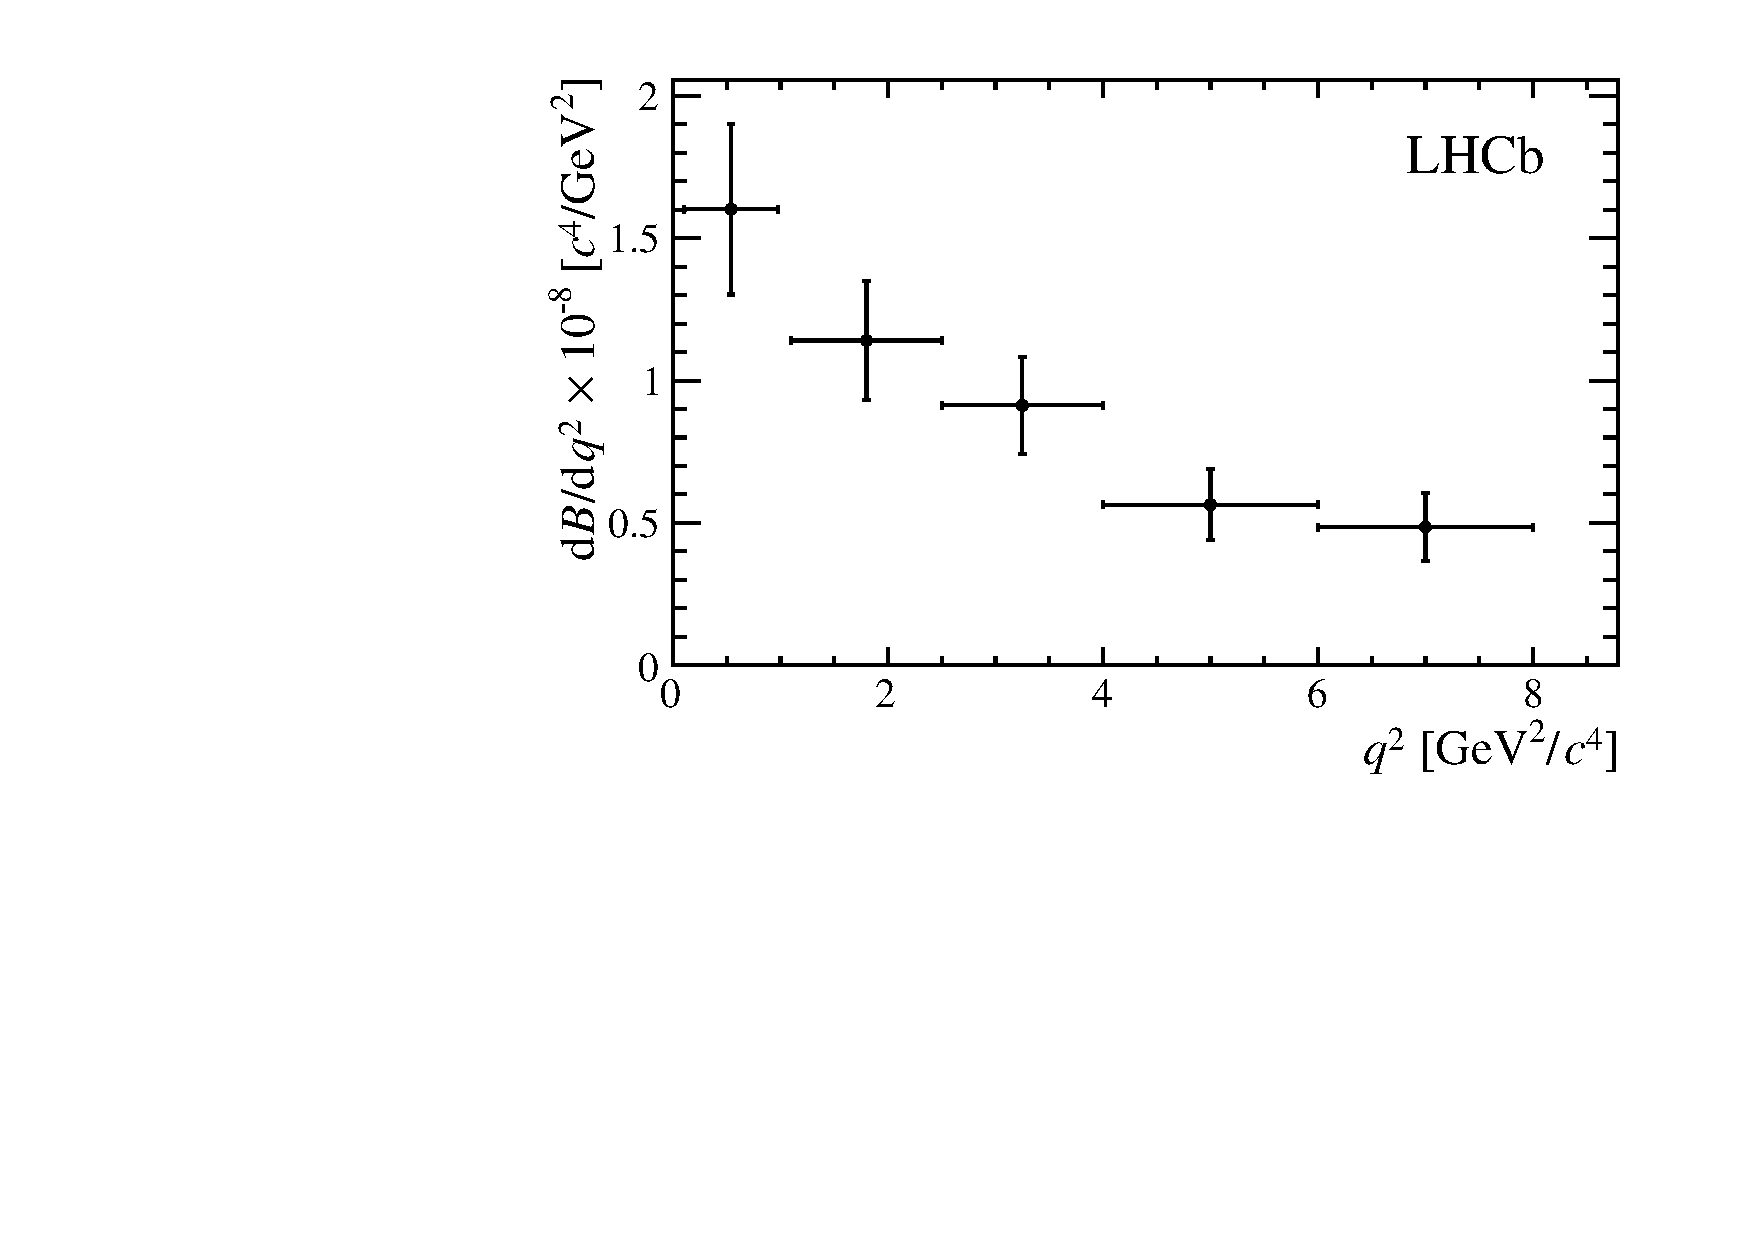
\includegraphics[width=0.7\textwidth]{figs/kpimm/bf/dbfdq2.pdf}
\caption{Differential branching fraction of \BdToKpimm in bins of \qsq. The uncertainties shown are the quadratic sum of the statistical and systematic uncertainties.}
\label{fig:bf}
\end{figure}
 
\begin{table}[!tb]
\caption{Differential branching fraction of \BdToKpimm in bins of \qsq. The first uncertainty is statistical, the second systematic and the third due to the uncertainty on the \BdToJPsiKstP and $\decay{\jpsi}{\mumu}$ branching fractions.}
\label{tab:bf}
\begin{center}
\begin{tabular}{lc}
\qsq [\gevgevcccc] & $\deriv\BF/\deriv\qsq \times 10^{-8}~[c^{4}/\gev^{2}]$ \\
\hline
$[0.10,0.98]$ & 1.48 $\pm$ 0.23 $\pm$ 0.03 $\pm$ 0.10 \\
$[1.10,2.50]$ & 1.13 $\pm$ 0.18 $\pm$ 0.02 $\pm$ 0.08 \\
$[2.50,4.00]$ & 0.94 $\pm$ 0.16 $\pm$ 0.03 $\pm$ 0.06 \\
$[4.00,6.00]$ & 0.61 $\pm$ 0.12 $\pm$ 0.02 $\pm$ 0.04 \\
$[6.00,8.00]$ & 0.49 $\pm$ 0.12 $\pm$ 0.01 $\pm$ 0.03 \\
\hline
$[1.10,6.00]$ & 0.84 $\pm$ 0.08 $\pm$ 0.02 $\pm$ 0.06 \\
\end{tabular}
\end{center}
\end{table}